\section{Method}
\label{sec.method}

In this section, we describe both the algorithmic design of agentic reasoning and the system design of the Confucius SDK that supports it. We first introduce the overarching design philosophy (AX, UX, DX) (\Cref{sec.3x}), then separate the presentation into (i) the SDK abstractions that realize these design choices in a modular and extensible manner and how they are instantiated on CCA (\Cref{sec.feat}) and (ii) the core agentic algorithms that govern how agents reason and improve over time (\Cref{sec.agentic_algo}). 

\subsection{Design Philosophy: AX, UX, and DX}
\label{sec.3x}

% \begin{wrapfigure}{r}{0.45\columnwidth}
%   \centering
%   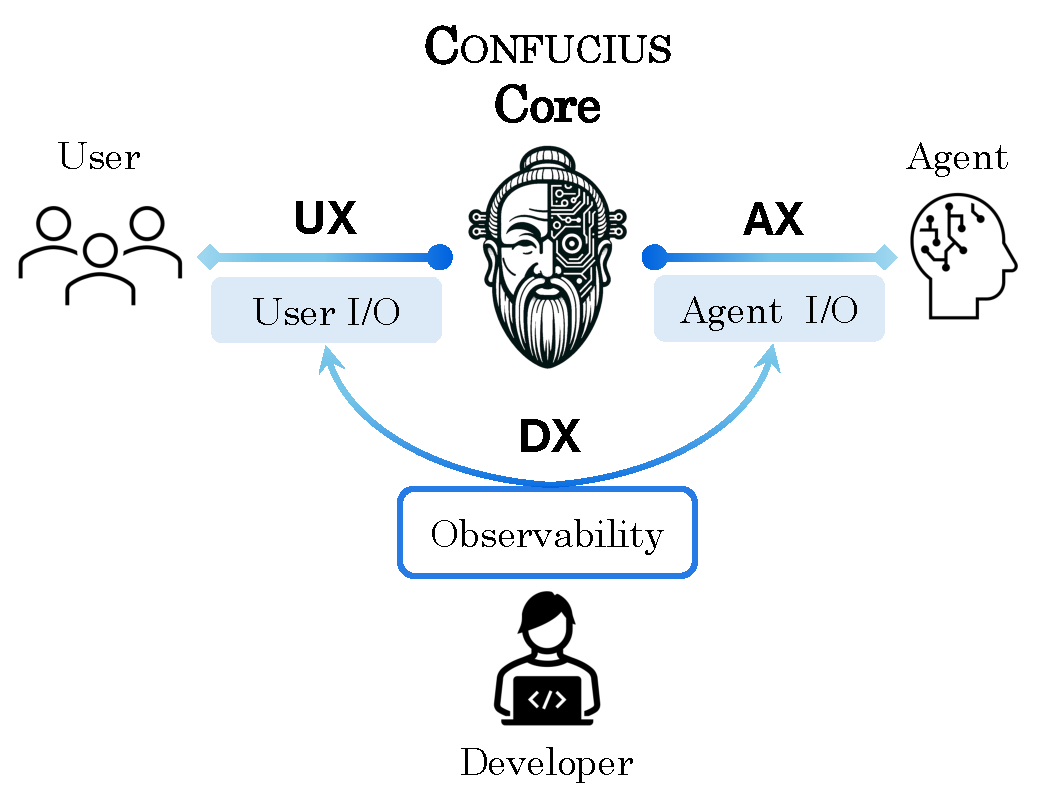
\includegraphics[width=\linewidth]{figs/3X.pdf}
%   \caption{Wrapped figure}
% \end{wrapfigure}

Most agent frameworks optimize for a single audience (users, agents, or developers). In contrast, the Confucius SDK adopts a three-axis philosophy that treats \emph{Agent Experience (AX)}, \emph{User Experience (UX)}, and \emph{Developer Experience (DX)} as distinct yet coupled design goals.
AX concerns the agent’s cognitive workspace: what context the model receives, how it is structured, and how it invokes tools. It should be concise and structured to avoid distraction or bias.
UX governs how humans observe and interact with the system, prioritizing transparency via readable logs, traces, and artifact previews.
DX supports building and improving agents through observability and control over prompts, tools, and memory, with visibility into both AX and UX.

Many systems conflate AX and UX by feeding human-facing traces directly to the model, causing context bloat, spurious anchors, and brittle debugging. CCA instead separates channels: users get rich instrumented traces, the agent gets compressed structured inputs, and developers can inspect and modify both.

Below shows a concrete example of the distinction between AX and UX: \\

\noindent
\begin{tcolorbox}[
  width=\columnwidth,
  colback=white,
  colframe=black!25,
  boxrule=0.4pt,
  arc=2pt,
  left=4pt,right=4pt,top=4pt,bottom=4pt,
  breakable
]
\textbf{For UX (Users See):}
\vspace{2pt}
\begin{lstlisting}[style=colcode]
Creating file at config.py
File created successfully at config.py
Here is the diff:
+ PORT=8080
+ DEBUG=true
+ MAX_CONNECTIONS=100
\end{lstlisting}

\vspace{0.4em}
\hrule
\vspace{0.4em}

\textbf{For AX (Agent Sees):}
\vspace{2pt}
\begin{lstlisting}[style=colcode]
Human: [previous user message]
AI: <file_edit type="create" file_path="config.py">...</file_edit>
Human: <result>File created successfully</result>
\end{lstlisting}
\end{tcolorbox}

In this case, users are presented with rich, streaming updates, whereas the agent receives only a compressed summary of the outcome stored in the memory manager, without the lengthy file diff message.


\subsection{Confucius SDK Features \& Instantiations on CCA}
\label{sec.feat}

\subsubsection{Context Management}
\label{sec.context_management}



Running agents on large-scale repositories quickly stresses even long-context LLMs: long debugging sessions, multi-file refactors, and nested tool calls all contribute to unbounded conversation growth. In many existing coding agent frameworks, agents either accumulate a single flat history (risking hard context limits and ``forgotten'' early decisions) or rely on naive truncation and ad-hoc retrieval, which can silently drop important information and are difficult to tune for different workloads. 
The Confucius SDK addresses this by providing an explicit \emph{agent context management} layer that combines hierarchical working memory with adaptive context compression.

\begin{figure*}[t]
    \centering
    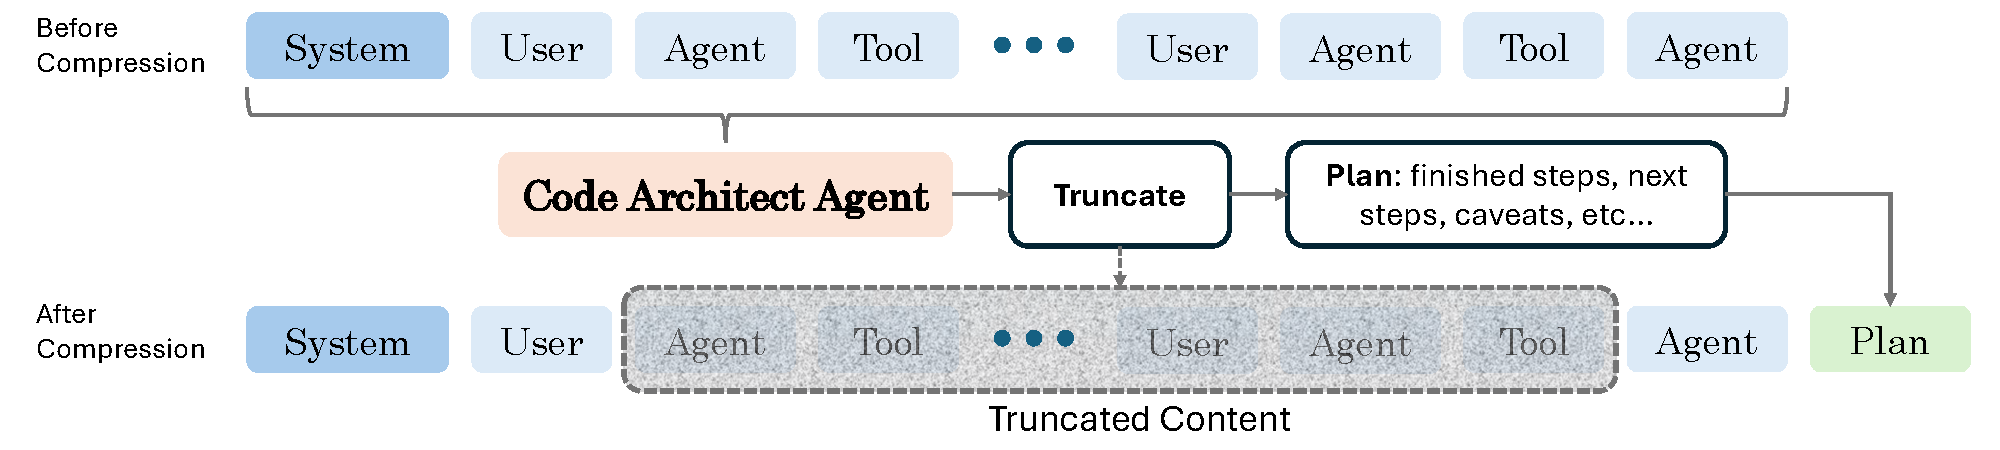
\includegraphics[width=\textwidth]{figs/mem_compress.pdf}
    \caption{\textbf{Context compression overview.}
    When the context window approaches configurable thresholds, the \textit{Architect} agent summarizes earlier turns into a structured plan containing goals, decisions, errors, and open TODOs. These compressed summaries replace original large spans of history while preserving a short window of recent interactions, enabling the agent to sustain multi-step reasoning over long trajectories without exceeding context limits.}
    \label{fig:mem_compress}
\end{figure*}

At the SDK level, each instantiated agent is backed by a file-system-based \textbf{hierarchical working memory} with configurable visibility scopes (e.g., session, entry, runnable). 
The memory is organized as a tree-structured namespace where internal nodes represent semantic groupings and leaf nodes store Markdown documents annotated with metadata tags. Agents interact with this memory through a set of primitive operations, including search, read, write, edit, and delete, which are exposed as callable tools during generation.
Below is an example of a constructed hierarchical memory of CCA on a SWE-Bench-Pro instance. 
The agent maintains this hierarchy throughout execution so that when context is pruned, important insights and intermediate artifacts can be stored and later retrieved efficiently:

\begin{tcolorbox}[colback=white,  % background color
                   colframe=black,    % frame color
                   coltext=metablue,      % text color
                   breakable,
                   fontupper=\scriptsize\fontfamily{pcr}\selectfont]  % font style and size
\begin{verbatim}
+-- instance_qutebrowser__qutebrowser-c09e1439...
    +-- hierarchical_memory_3a7488c6-bf8c-11f0-...
        +-- qutebrowser_process_cleanup
            |-- analysis.md
            |-- implementation_summary.md
            +-- todo.md
\end{verbatim}
\end{tcolorbox}


On top of this hierarchy, Confucius SDK integrates an adaptive \textbf{context compression} mechanism (\Cref{fig:mem_compress}) driven by an \emph{Architect Agent}. When the context length approaches configurable thresholds, the Architect Agent is invoked in a separate call to analyze the conversation history and construct a structured summary that explicitly preserves key information categories (e.g., task goals, decisions made, open TODOs, and critical error traces). The system then replaces marked historical messages with this compressed summary while maintaining a rolling window of recent messages in their original form. The summary is inserted as a new message, and all future turns will see both the compact summary and the recent raw history. 

This context management design provides two key benefits.
First, structured summarization triggered only when needed preserves semantically important information and maintains access to long reasoning chains, avoiding the brittleness of fixed-window truncation or simple retrieval.
Second, the hierarchical memory stores and refines key insights throughout execution, complementing the summaries and ensuring that important state persists even as the raw history is compressed.
In CCA, these mechanisms are essential for handling long-running software engineering sessions on industrial-scale codebases, improving performance on long-context coding tasks without requiring changes to the underlying orchestrator or extensions. 
Similar context engineering techniques are also reported in recent production-level LLMs \citep{anthropic2025contextengineering, openai2025sessionmemory}.


\subsubsection{Note-Taking}
\label{sec.note_taking}

Flat chat logs are not an ideal representation for long-term memory: they are verbose and difficult to reuse without manually rereading entire transcripts. In typical frameworks, any cross-session ``memory'' is either absent or implemented via coarse-grained embeddings over whole turns, which tends to miss important structure such as architectures, design decisions, and failure modes. To support agents that improve over time and can pick up long-running projects where they left off, the Confucius SDK includes an explicit \emph{note-taking} mechanism that memorizes interaction traces as structured persistent knowledge.

At the SDK level, every interaction session is logged into a structured ``trajectory'', including user messages, tool invocations, LLM outputs, and system events. A dedicated \textbf{note-taking agent} can distill these trajectories into compact notes without affecting the online latency of the primary agent. Persistent notes are stored as Markdown files in a file-system-like tree: each session has an associated directory, under which the note-taking agent can create paths such as \texttt{research/findings.md} and  \texttt{solutions/bug\_fix.md}. Leaves in this hierarchy are Markdown documents with lightweight tags, maintained as typed memory nodes. The SDK exposes structured tools to search, read, write, edit, delete, and import these nodes, so notes can be programmatically updated and reused across sessions. Examples of taken notes are shown in Appendix~\ref{app:notes}.

A distinctive aspect of the Confucius SDK’s note-taking is its emphasis on \emph{hindsight notes} for failures. The note-taking layer encourages agents to record not only successful solutions but also compilation errors, runtime exceptions, and unproductive strategies, together with eventual resolutions or reasons for abandonment. Over time, this yields a corpus of failure cases indexed by error messages, stack traces, and affected components. When a similar failure appears in a future session, an agent can retrieve the corresponding hindsight note and immediately surface known fixes or workarounds, rather than rediscovering them from scratch. In CCA, these mechanisms turn day-to-day usage on large codebases into a steadily growing, human-readable body of durable knowledge that improves continuity across sessions and reduces repeated “thrashing” on recurring issues.



\subsubsection{Extensions}
\label{sec.extensions}

The Confucius SDK implements output parsing, tool invocation, and side-effect management via \emph{extensions}: modular components that attach to the orchestrator and run at every execution step. Whereas many frameworks hard-code these behaviors in ad-hoc logic or model-specific prompting, Confucius exposes them as first-class, composable modules that are easier to reuse, audit, and adapt.

Each extension is a typed configuration object that registers ordered callbacks (e.g., \texttt{on\_input\_messages}, \texttt{on\_llm\_output}) executed within the orchestrator loop. Callbacks share a run context providing I/O, session state, memory, and artifacts, enabling extensions to shape prompts, interpret structured outputs (XML tags or native tool calls), and inject or filter messages while maintaining local state.

Conceptually, extensions cover perception, reasoning, and action: they (i) parse and validate model outputs into structured actions, (ii) rewrite or annotate inputs before LLM calls, and (iii) execute tools (e.g., shell, file edits) and summarize results into memory or artifacts. By routing tool use and prompt shaping through extensions, Confucius cleanly separates orchestration from capabilities. CCA is thus an orchestrator paired with a particular extension bundle; our ablations (\Cref{tab:context_mgmt}) vary only enabled extensions and configurations while holding the loop fixed, so improvements to extensions transfer across all Confucius-based agents.



\subsection{Agentic Algorithms: Orchestration and Automatic Agent Development}
\label{sec.agentic_algo}

\subsubsection{The Confucius Orchestrator}
\label{sec.orchestrator}

\begin{wrapfigure}{r}{0.6\textwidth}
\vspace{-2em}
\begin{tcolorbox}[
    enhanced,
    colback=white,
    colframe=black!40,
    sharp corners,
    boxrule=0.5pt,
    left=4pt,
    right=4pt,
    top=4pt,
    bottom=4pt
]

\hrule height 0.8pt \vspace{0.3em}

\textbf{Algorithm 1: Confucius Orchestrator Loop}

\hrule height 0.4pt \vspace{0.3em}

\begin{algorithmic}[1]
    \State \textbf{Initialize} session context, memory, extensions
    \While{iteration $< \texttt{max\_iters}$}
        \State \textbf{Invoke} LLM with system prompt + memory
        \State \textbf{Parse} LLM output into actions
        \ForAll{actions $a$}
            \State \textbf{Route} $a$ to its extension
            \State \textbf{Execute} extension; update memory
            \If{extension signals continuation}
                \State add observations (results, error, etc.) to memory
                \State \textbf{continue}
            \EndIf
        \EndFor
        \State \textbf{Check} for completion; \textbf{break} if done
    \EndWhile
    \State \textbf{return} final output and artifacts
\end{algorithmic}

\hrule height 0.4pt

\end{tcolorbox}
\vspace{-2em}
\end{wrapfigure}

% \begin{algorithm}[tb]
%    \caption{Confucius Orchestrator Loop}
%    \label{alg:confucius_orchestrator}
% \begin{algorithmic}[1]
%    \STATE \textbf{Initialize} session context, memory, and extensions.
%    \WHILE{iteration $< \texttt{max\_iters}$}
%       \STATE \textbf{Invoke} LLM with system prompt and memory.
%       \STATE \textbf{Parse} LLM output into actions.
%       \FORALL{actions $a$}
%          \STATE \textbf{Route} $a$ to its extension.
%          \STATE \textbf{Execute} extension and update memory.
%          \IF{extension signals continuation}
%             \STATE Add observations (e.g. errors) to memory.
%             \STATE \textbf{continue}
%          \ENDIF
%       \ENDFOR
%       \STATE \textbf{Check} for completion; \textbf{break} if done.
%    \ENDWHILE
%    \STATE \textbf{return} final output and artifacts.
% \end{algorithmic}
% \end{algorithm}


The Confucius Orchestrator is a minimal, extensible loop that repeatedly calls the LLM, interprets its outputs, and coordinates tool execution. The same orchestrator is reused across all Confucius SDK agents; CCA is one configuration of this loop with coding-oriented extensions enabled.

\paragraph{Output Processing.}
The orchestrator supports two LLM interfaces: (1) native tool-use models emit structured tool calls that are routed to extension handlers; (2) other models emit XML-style tags (e.g., \texttt{<bash>...</bash>}), which are parsed into the same action representation. This preserves broad model compatibility while leveraging native tool-use when available.

\paragraph{Iteration Control.}
Execution is bounded by a maximum iteration cap, but termination is typically agent-driven. Each iteration parses the LLM output into actions; if no further actions are produced, the run ends. Extensions can also force continuation (e.g., a bash execution returns an interrupt with command output), causing the orchestrator to re-invoke the LLM with updated context. Together, these mechanisms support multi-step reasoning and tool use within safe bounds.



\subsubsection{Meta-agent: A Build-Test-Improve Loop}
\label{sec.meta_agent}


A recurring limitation of existing agent frameworks is that agent behavior is largely \emph{static}: humans hand-design prompts, tool wiring, and guardrails, then periodically revise them by trial and error. This is labor-intensive and does not scale with growing tool ecosystems. Moreover, we find that naive implementations of file-editing or command-line tools, even when they are functionally correct, often underperform because the surrounding prompts and error-handling conventions are not tuned to realistic workloads. We address this by introducing a \emph{Meta Agent}, an agent that automatically builds and refines other agents through an explicit \emph{build-test-improve} loop, turning agent design itself into an agentic, evaluation-driven automatic process.
More implementation details of Meta Agent can be found at Appendix \ref{sec.meta-agent-details}.

This Meta-agent capability lives at the Confucius SDK level but directly benefits CCA. The proposed CCA is itself the outcome of the Meta-agent's build-improve-test loop: we start from a high-level description of a repository-level software engineering assistant, let the Meta-agent synthesize the orchestrator configuration, tool wiring, and prompts, and then repeatedly refine them against a production-grade test set until performance stabilizes. 
% The resulting agent exhibits more reliable tool selection and recovery behaviors than our initial hand-written designs, and these improvements are reflected in the tool-use ablations reported in \Cref{sec:meta-agent-tool-use}.
% At the same time, the same Meta-agent interface allows users to rapidly spin up use-case-specific agents using this automated iteration loop.
% extending this process to a broader family of specialized agents is an active direction for future work.

